\subsection{trie.go} 

The data structure defined here is \emph{trie}, that is used to build a tree. It contains a byte (used as index), interface and two trie type pointers (one to the child and the other to the sibling).\\
Here the functions of \emph{trie} type:

\begin{itemize}

\item \emph{func (t *trie) prefix(b []byte) (s []byte, r *trie)}\\
It finds the longest present prefix of b. It returns the prefix and pointer to a trie variable that is the last node whose index matches the prefix or \emph{t} if there is no matching index in \emph{t's} children.

\item \emph{func (t *trie) Lookup(key []byte) (value interface{}, ok bool)}\\
It looks up for a key in \emph{t} variable. If the key doesn't exist or the interface returned by prefix function is nil, it returns \emph{nil} and \emph{false}, otherwise, it returns the interface and \emph{true}.

\item \emph{func (t *trie) Insert(key []byte, value interface{})}\\
It inserts a new interface using the key received as parameter. If the key already exists, it updates the interface value.

\item \emph{func (t *trie) Delete(key []byte)}\\
It deletes an interface by setting it to nil according to the key received as parameter. It searches and records the deepest node with multiple children and siblings.

\end{itemize}

\begin{figure}[H]
\centering
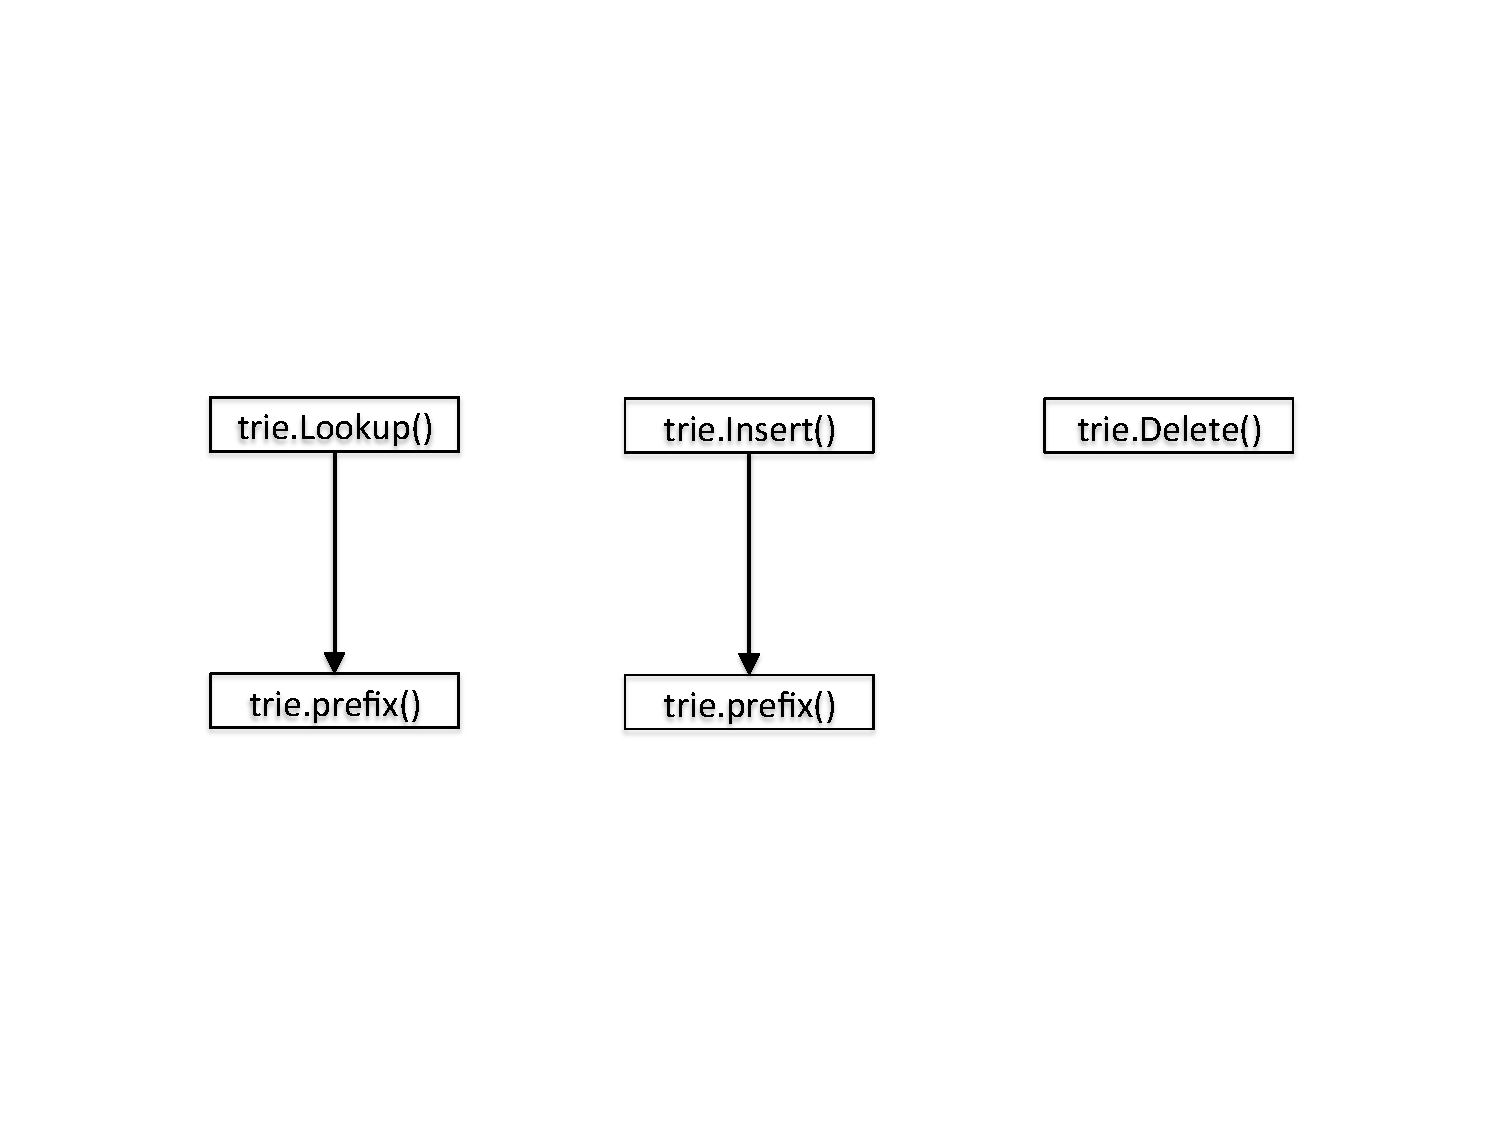
\includegraphics[scale=0.50]{triePackage}
\caption{trie.go package}
\end{figure}